\chapter{Analiza wyników}
\label{cha:analiza_wynikow}

Ostateczny model klasyfikatora po dobraniu odpowiedniej architektury i dostrojeniu parametrów został przetrenowany przez 36 epok, a ostatnia poprawa wartości funkcji błedu nastąpiła w 29 epoce. Przebieg procesu uczenia został przedstawiony na rysunku \ref{fig:trening_model_4}. Krzywa walidacji prawie w każdym punkcie nadąża za krzywą uczenia, co oznacza stabilność algorytmu. Wartość skuteczności modelu na zbiorze testowym wynosi 85\% (\ref{tab:acc}).

\begin{figure}[h!]
	\centering
	\centering
		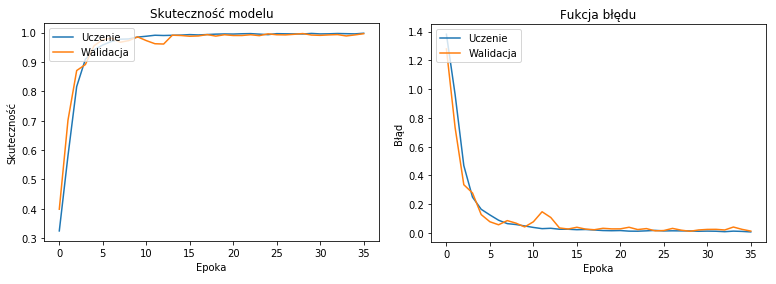
\includegraphics[scale=0.5]{trening_model_4}	
	\caption{Zależność skuteczności i błędu od epoki w procesie uczenia opracowanego klasyfikatora.}\label{fig:trening_model_4}
\end{figure}

\begin{table}[h!]
\centering
\caption[Short Heading]{Skuteczność opracowanego klasyfikatora.}
\label{tab:acc}
\begin{tabular}{|c|c|c|c|}
\hline
\textbf{typ zbioru}           & \textbf{treningowy} & \textbf{walidacyjny} & \textbf{testowy} \\ \hline
\textbf{skuteczność {[}\%{]}} & 99                  & 99                   & 85               \\ \hline
\end{tabular}
\end{table}

{\parindent0pt
Do klasyfikacji używany jest model uczony przez 29 epok. Dane wejściowe są w obrazami RGB o wymiarach 120x160, przeskalowanymi do zakresu wartości pikseli 0-1. Ramki podzielone są na porcje po 32 obrazy, co daje 248 iteracji w każdej epoce uczenia zgodnie ze wzorem (\ref{equ:iter_num_trening}). Testowanie odbywa się w 62 iteracjach, zgodnie ze wzorem (\ref{equ:iter_num_test}). Takie podejście pozwala na przejście wszystkich danych przez system w każdej epoce, zarówno podczas uczenia, jak i testowania. Wynik dla zbioru testowego jest nieznacznie niższy niż przed kalibracją, ale w zamian uzyskano gwarancję, że wynik ten będzie powtarzalny, gdyż ustabilizowano proces uczenia. 

\begin{equation}
i = \floor*{\frac{x}{b}} = \floor*{\frac{7965}{32}} = 248
\label{equ:iter_num_trening}
\end{equation}
gdzie,
\begin{eqwhere}[2cm]
	\item[$i$] ilość iteracji w jednej epoce treningu,
	\item[$x$] ilość ramek treningowych,
	\item[$b$] ilość ramek w porcji.
\end{eqwhere}

\begin{equation}
j = \floor*{\frac{y}{b}} = \floor*{\frac{1992}{32}} = 62
\label{equ:iter_num_test}
\end{equation}
gdzie,
\begin{eqwhere}[2cm]
	\item[$j$] ilość iteracji teście,
	\item[$y$] ilość ramek testowych,
	\item[$b$] ilość ramek w porcji.
\end{eqwhere}

Na podstawie ogólnej macierzy pomyłek (\ref{tab:general_conf_matrix}) można wyprowadzić macierze dla każdej klasy osobno i wyprowadzić parametry pozwalające na dokładniejszą analizę jakości klasyfikacji. Struktura takiej macierzy zakłada binarność problemu dla każdej klasy, gdzie wynikiem jest potwierdzenie lub odrzucenie przynależności do danej klasy (\ref{tab:bin_conf_matrix}).

\begin{table}[h!]
\centering
\caption[Short Heading]{Macierz pomyłek zbioru testowego opracowanego klasyfikatora.}
\label{tab:general_conf_matrix}
\begin{tabular}{|c|c|c|c|c|c|}
\hline
\textbf{}                           & \multicolumn{5}{c|}{\textbf{predykcja}} \\ \hline
{\multirow{5}{*}{\rotatebox[origin=c]{90}{\textbf{klasa}}}} &         & E       & L        & M      & N       \\ \cline{2-6} 
                                    & E       & 141       & 144      & 141     & 197      \\ \cline{2-6} 
                                    & L       & 134       & 149      & 130      & 207      \\ \cline{2-6} 
                                    & M       & 145       & 128      & 141      & 206      \\ \cline{2-6} 
                                    & N       & 140       & 137      & 140      & 207       \\ \hline
\end{tabular}
\end{table}

\begin{table}[h!]
\centering
\caption[Short Heading]{Ogólna macierz pomyłek zbioru testowego dla danej klasy.}
\label{tab:bin_conf_matrix}
\begin{tabular}{|c|c|c|c|c|c|}
\hline
\textbf{}                           & \multicolumn{3}{c|}{\textbf{klasa predykowana}} \\ \hline
{\multirow{3}{*}{\rotatebox[origin=c]{90}{\textbf{klasa rzeczywista}}}} &         & klasa pozytywna      & klasa negatywna  \\ \cline{2-4} 
                                    & stan       & prawdziwie dodatnia     & fałszywie ujemna   \\
                                    & pozytywny       & (ang. \textit{true positive}, TP)      & (ang. \textit{false negative}, FN)     \\ \cline{2-4} 
                                    & stan       & fałszywie dodatnia      & prawdziwie ujemna  \\
                                    & negatywny       & (ang.\textit{false positive}, FP)     & (ang. \textit{true negative}, TN)               \\ \hline
\end{tabular}
\end{table}


Na podstawie wartości w tabeli \ref{tab:bin_conf_matrix} przygotowano szczegółowe tabele dla poszczególnych klas (\ref{tab:E_bin_conf_matrix}, \ref{tab:L_bin_conf_matrix}, \ref{tab:M_bin_conf_matrix}, \ref{tab:N_bin_conf_matrix}). Następnie zostały obliczane i umieszczone w tabeli \ref{tab:params_test} takie parametry klasyfikatora jak: 
\begin{itemize}
\item skuteczność (ACC) (\ref{equ:acc}),
\begin{equation}
ACC = \frac{TP + TN}{P + N}
\label{equ:acc}
\end{equation}

\item precyzja (PPV) (\ref{equ:ppv}),
\begin{equation}
PPV = \frac{TP}{TP + FP}
\label{equ:ppv}
\end{equation}

\item czułość (TPR) (\ref{equ:tpr}),
\begin{equation}
TPR = \frac{TP}{TP + FN}
\label{equ:tpr}
\end{equation}

\item swoistość (SPC) (\ref{equ:spc}),
\begin{equation}
SPC = \frac{TN}{FP + TN}
\label{equ:spc}
\end{equation}

\item miara F1 (\ref{equ:f1}),
\begin{equation}
F1 = 2 \frac{PPV \cdot TPR}{PPV + TPR}
\label{equ:f1}
\end{equation}
\end{itemize}

\begin{table}[h!]
\centering
\caption[Short Heading]{Macierz pomyłek zbioru testowego dla klasy E.}
\label{tab:E_bin_conf_matrix}
\begin{tabular}{|c|c|c|c|c|c|}
\hline
\textbf{}                           & \multicolumn{3}{c|}{\textbf{predykcja}} \\ \hline
{\multirow{3}{*}{\rotatebox[origin=c]{90}{\textbf{klasa}}}} &         & \textit{E}     & $\widetilde{E}$ \\ \cline{2-4} 
                                    & \textit{E}      & 141     & 482   \\ \cline{2-4} 
                                    & $\widetilde{E}$       & 419      & 1445   \\ \hline
\end{tabular}
\end{table}

\begin{table}[h!]
\centering
\caption[Short Heading]{Macierz pomyłek zbioru testowego dla klasy L.}
\label{tab:L_bin_conf_matrix}
\begin{tabular}{|c|c|c|c|c|c|}
\hline
\textbf{}                           & \multicolumn{3}{c|}{\textbf{predykcja}} \\ \hline
{\multirow{3}{*}{\rotatebox[origin=c]{90}{\textbf{klasa}}}} &         & \textit{L}     & $\widetilde{L}$ \\ \cline{2-4} 
                                    & \textit{L}      & 149     & 471   \\ \cline{2-4} 
                                    & $\widetilde{L}$       & 409      & 1458   \\ \hline
\end{tabular}
\end{table}

\begin{table}[h!]
\centering
\caption[Short Heading]{Macierz pomyłek zbioru testowego dla klasy M.}
\label{tab:M_bin_conf_matrix}
\begin{tabular}{|c|c|c|c|c|c|}
\hline
\textbf{}                           & \multicolumn{3}{c|}{\textbf{predykcja}} \\ \hline
{\multirow{3}{*}{\rotatebox[origin=c]{90}{\textbf{klasa}}}} &         & \textit{M}     & $\widetilde{M}$ \\ \cline{2-4} 
                                    & \textit{M}      & 141     & 479   \\ \cline{2-4} 
                                    & $\widetilde{M}$       & 411      & 1456   \\ \hline
\end{tabular}
\end{table}

\begin{table}[h!]
\centering
\caption[Short Heading]{Macierz pomyłek zbioru testowego dla klasy N.}
\label{tab:N_bin_conf_matrix}
\begin{tabular}{|c|c|c|c|c|c|}
\hline
\textbf{}                           & \multicolumn{3}{c|}{\textbf{predykcja}} \\ \hline
{\multirow{3}{*}{\rotatebox[origin=c]{90}{\textbf{klasa}}}} &         & \textit{N}     & $\widetilde{N}$ \\ \cline{2-4} 
                                    & \textit{N}      & 207     & 417   \\ \cline{2-4} 
                                    & $\widetilde{N}$       & 610      & 1253   \\ \hline
\end{tabular}
\end{table}

Precyzja klasyfikacji jest stosunkiem właściwych sklasyfikowań do całkowitej liczby przyporządkowań do danej klasy, podczas gdy czułość obliczana jest w stosunku do rzeczywistej liczebności danej klasy. Precyzja opisuje więc prawdopodobieństwo, że losowo wybrana ramka sklasyfikowana jako dana klasa naprawdę do tej klasy należy. Czułość opisuje prawdpodobieństwo, że losowo wybrana ramka z danej klasy zostanie przyporządkowana właśnie jako ta klasa. Wartością, która łączy obia te współczynniki jest miara F1. Swoistość jest to parametr, który opisuje prawdopodobieństwo wykrycia, że ramka nie należy do danej klasy. Im wyższe są wartości tych współczynników, tym lepszy klasyfikator.

\begin{table}[h!]
\centering
\caption[Short Heading]{Parametry mierzące jakość klasyfikacji na zbiorze testowym opracowanego klasyfikatora.}
\label{tab:params_test}
\begin{tabular}{|c|c|c|c|c|c|}
\hline
\textbf{Parametr}                              & \textbf{Liczba próbek} & \textbf{Precyzja} & \textbf{Czułość} & \textbf{Swoistość} & \textbf{Miara F1} \\ \hline
\textbf{klasa E} & 623 & 0.25   & 0.23   & 0.77 & 0.24  \\ \hline
\textbf{klasa L} & 620 & 0.27  & 0.24 & 0.78 & 0.25 \\ \hline
\textbf{klasa M}  & 620 & 0.26   & 0.23    & 0.78 & 0.24  \\ \hline
\textbf{klasa N}  & 624 & 0.25   & 0.33   & 0.67 & 0.29\\ \hline
\end{tabular}
\end{table}
}

\section{Wizualizacja działania}

Kolejne filry konwolucyjne są odpowiedzialne za znajdowanie coraz bardziej szczegółowych informacji w obrazie. W celu zbadania jak działa sieć neuronowa zwizualizowano filtry warstw konwolucyjnych dla obrazu z klasy E. Z tego powodu, że warstw konwolucyjnych jest aż 13 w niniejszej pracy zamieszczone zostają jedynie wybrane warstwy.

\begin{figure}[h!]
	\centering
	\centering
		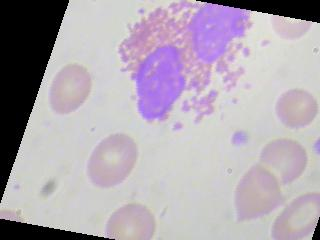
\includegraphics[scale=0.5]{E5}	
	\caption{Obraz z klasy E, dla którego zwizualizowano filtry na rysunku \ref{fig:filters_1}, \ref{fig:e_conv_148},   \ref{fig:e_conv_151},  \ref{fig:e_conv_154},  \ref{fig:e_conv_156}.}\label{fig:e_conv_148}
\end{figure}

\begin{figure}[h!]
    \centering
    \begin{subfigure}[b]{0.65\textwidth}
        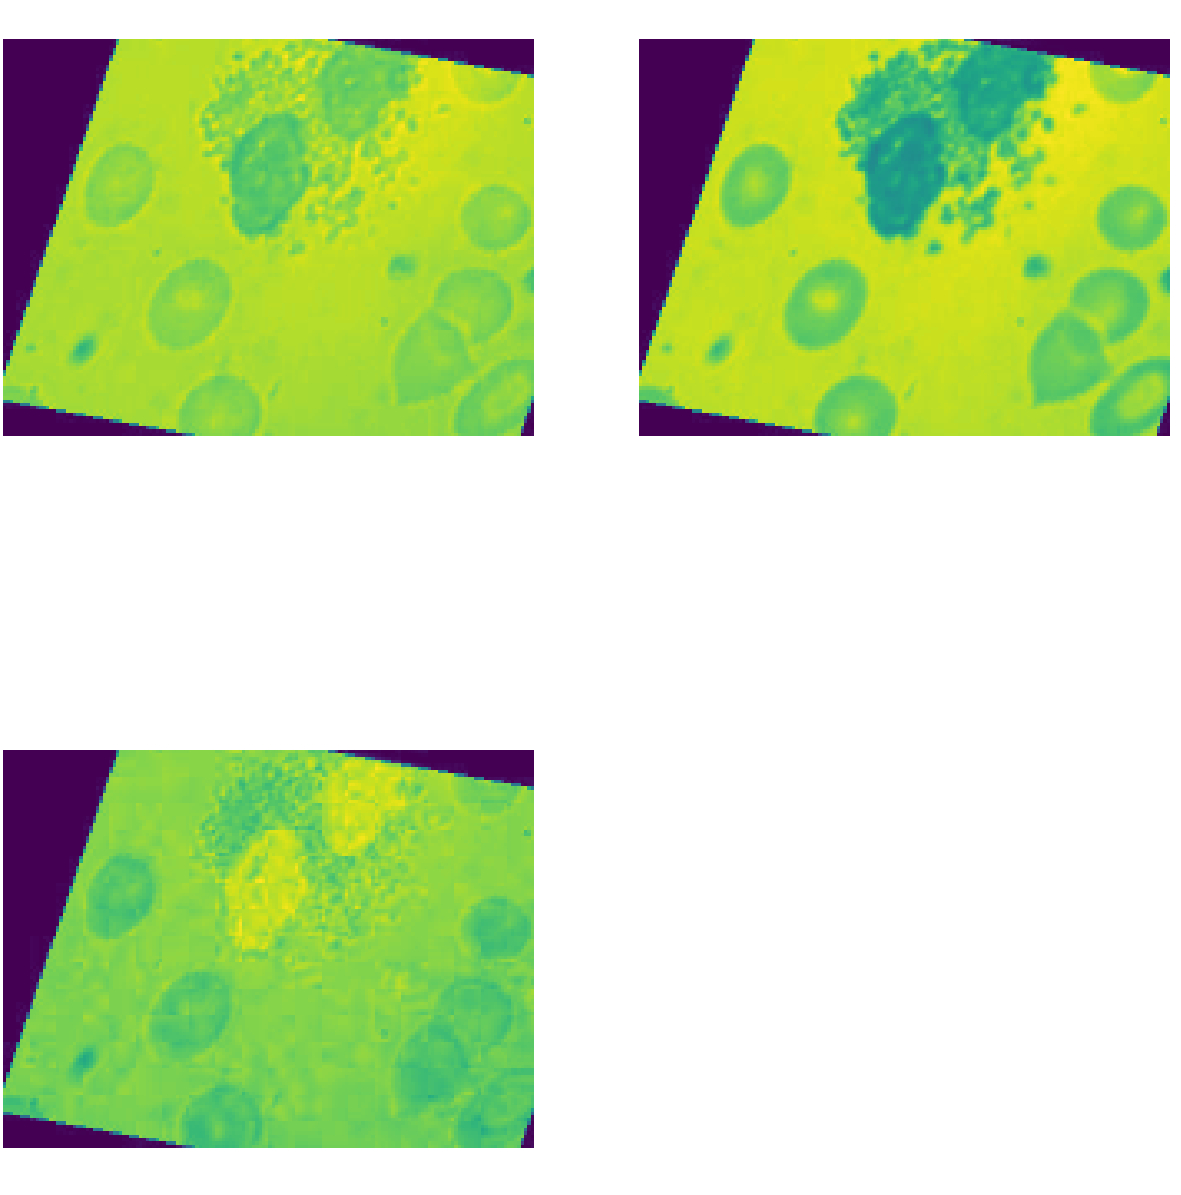
\includegraphics[width=\textwidth]{e_bn_output}\caption{}
        \label{fig:e_bn_output}
    \end{subfigure}
    \begin{subfigure}[b]{0.65\textwidth}
        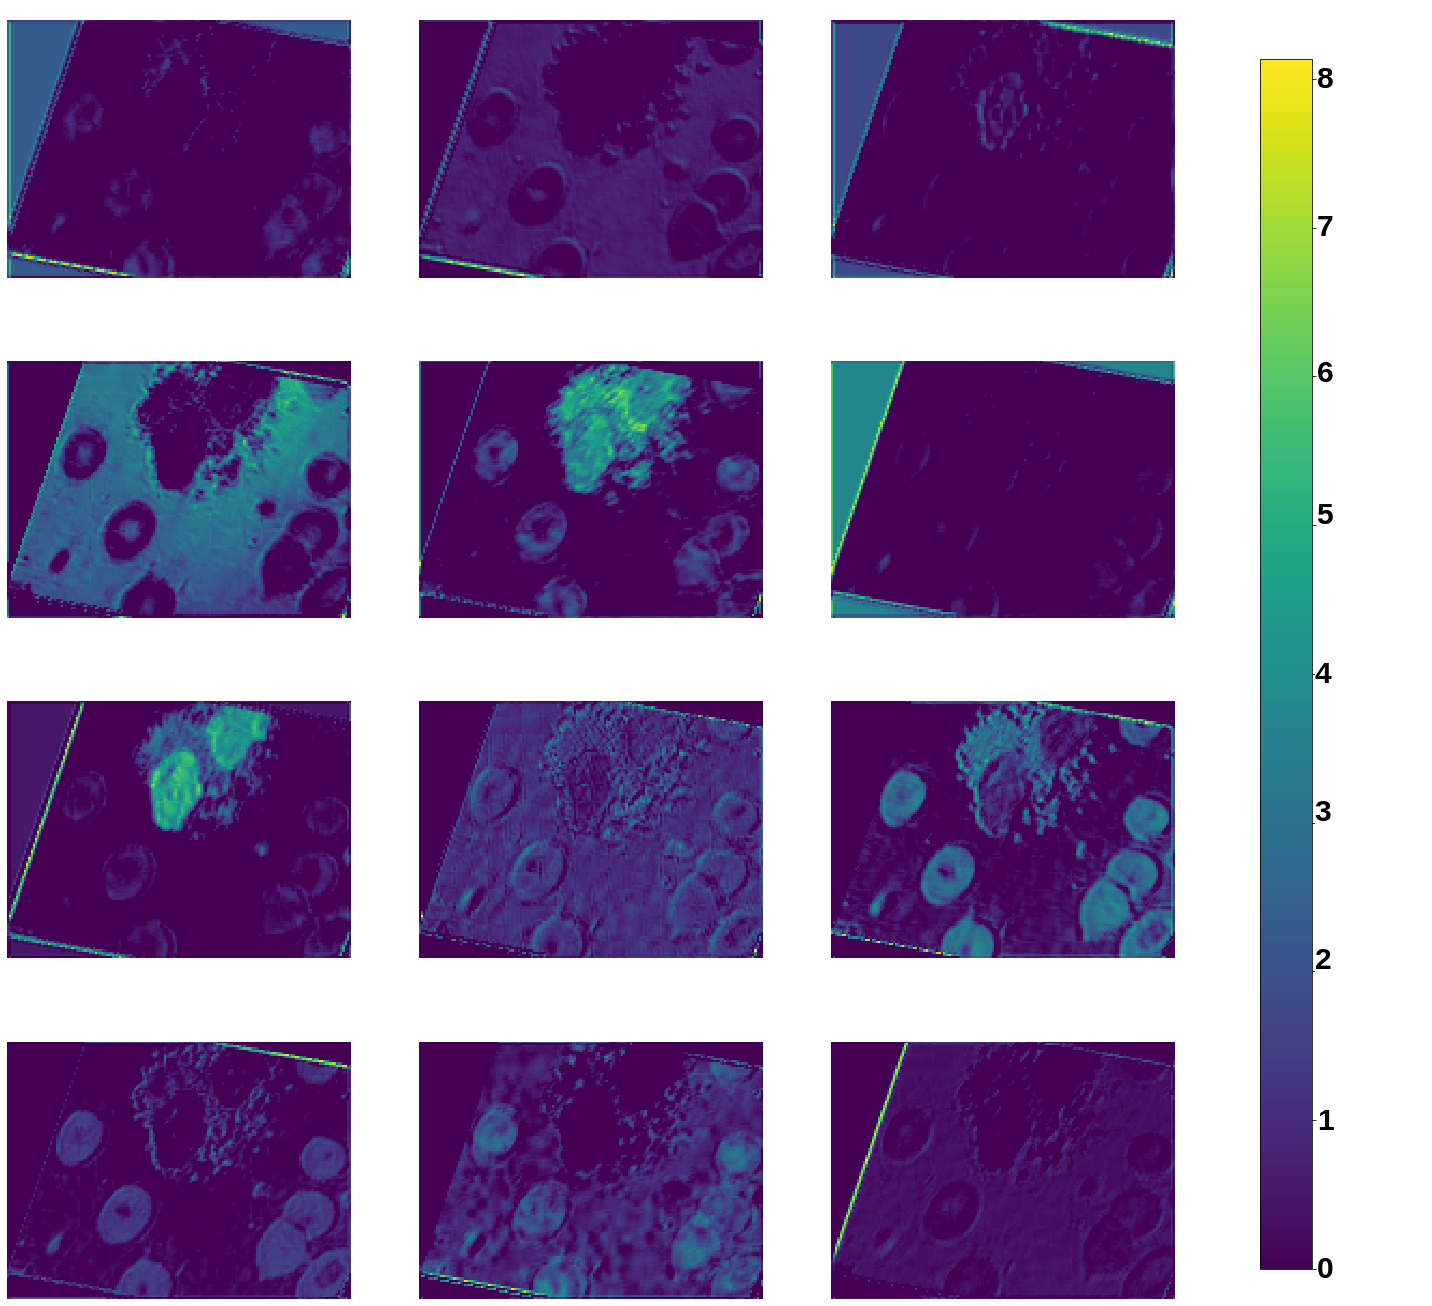
\includegraphics[width=\textwidth]{e_conv_145}\caption{}
        \label{fig:e_conv_145}
    \end{subfigure}
    \caption{Zdjęcia przedstawiające: \protect\subref{subfigure_a} dane wejściowe pierwszej warstwy konwolucyjnej po przejściu przez normalizację, \protect\subref{subfigure_b} filtry drugiej warstwy konwolucyjnej.}
	\label{fig:filters_1}
\end{figure}

\begin{figure}[h!]
	\centering
	\centering
		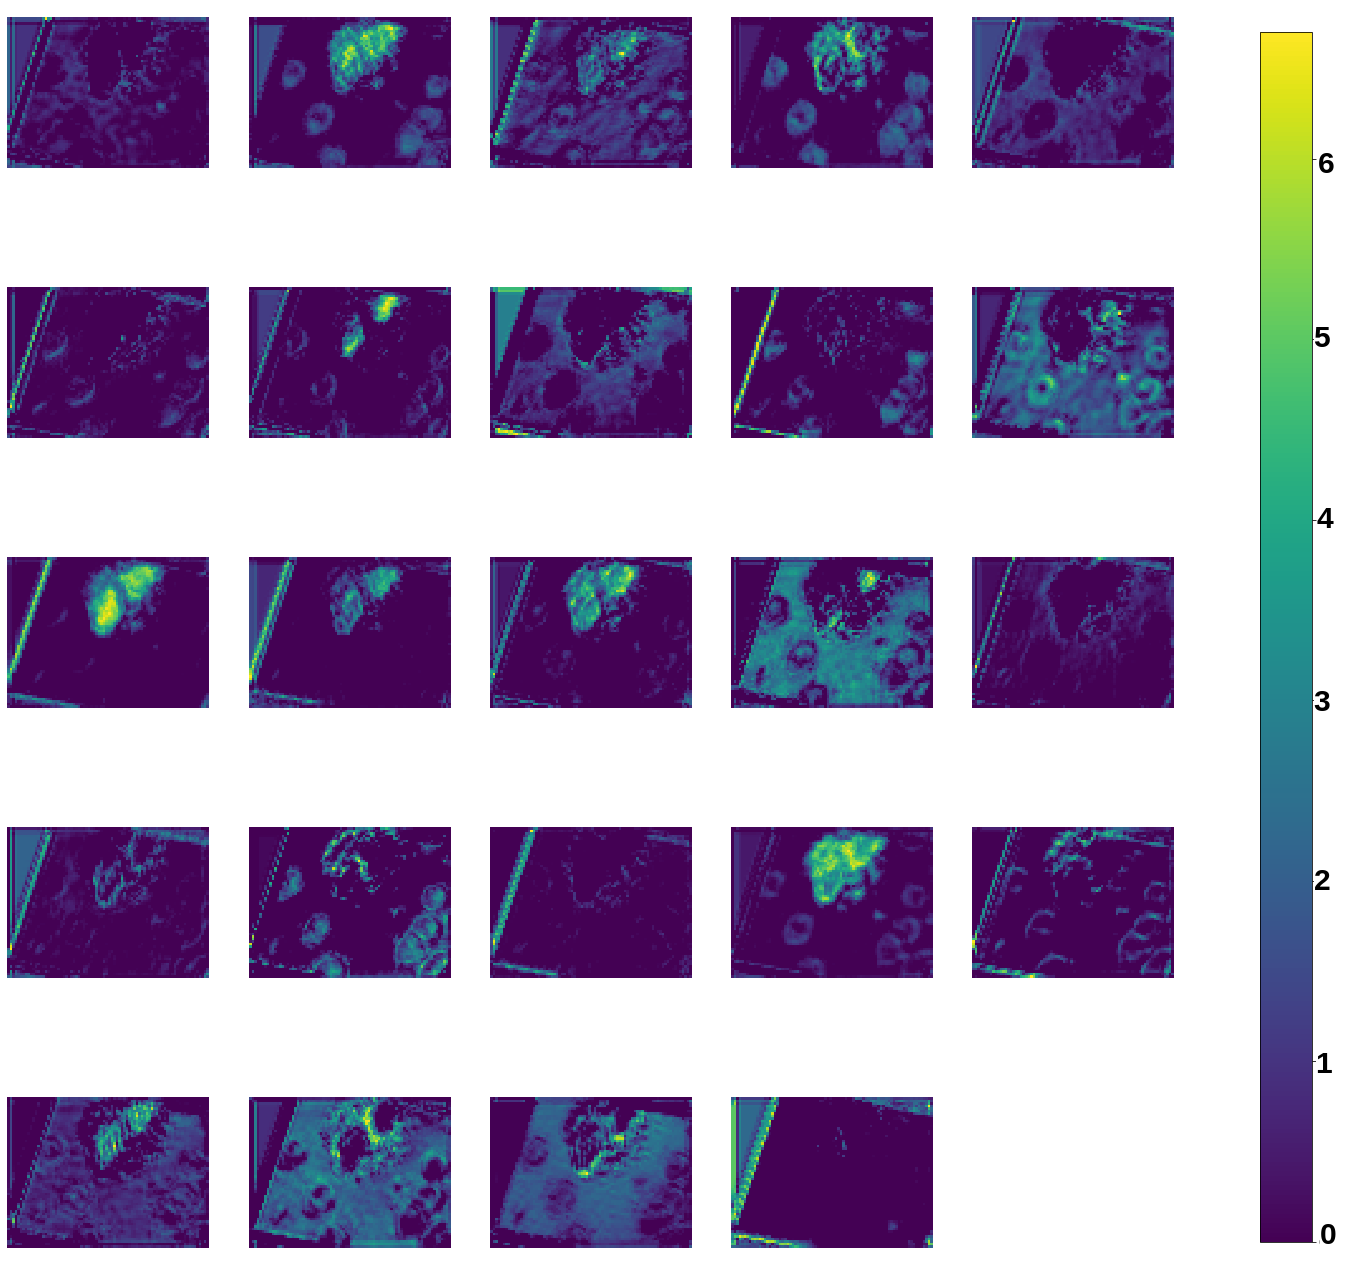
\includegraphics[scale=0.35]{e_conv_148}	
	\caption{Piąta warstwa konwolucyjna z 24 filtrami.}\label{fig:e_conv_148}
\end{figure}

\begin{figure}[h!]
	\centering
	\centering
		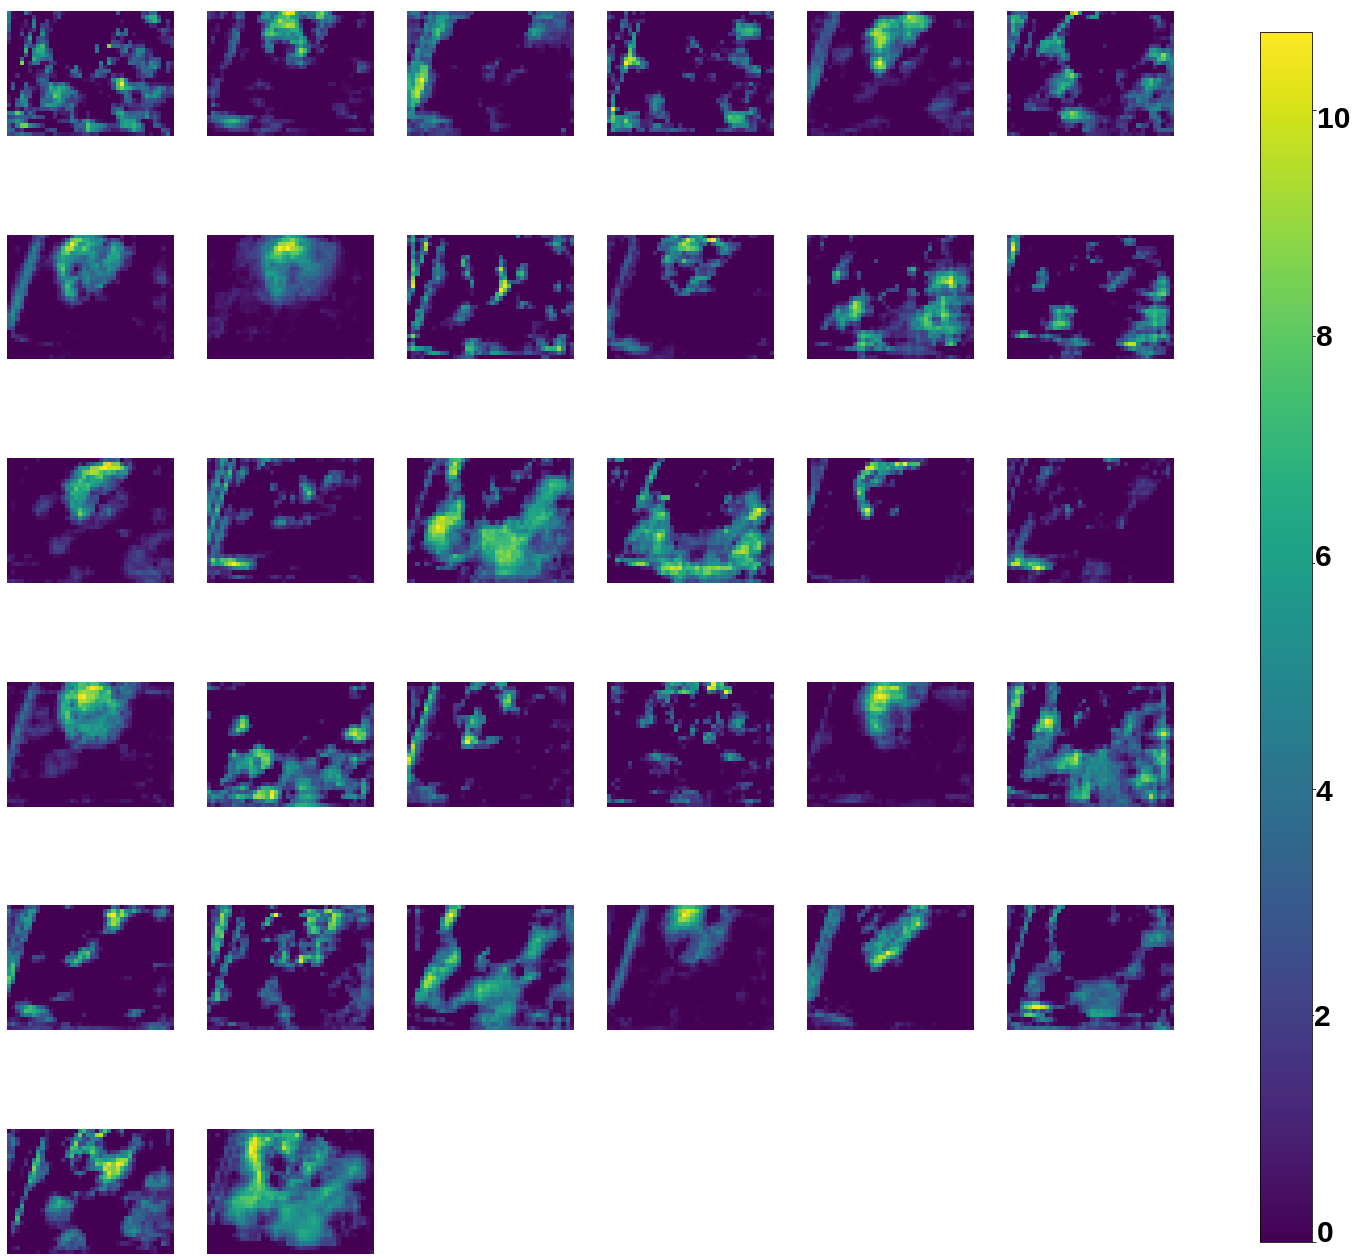
\includegraphics[scale=0.35]{e_conv_151}	
	\caption{Ósma warstwa konwolucyjna z 32 filtrami.}\label{fig:e_conv_151}
\end{figure}

\begin{figure}[h!]
	\centering
	\centering
		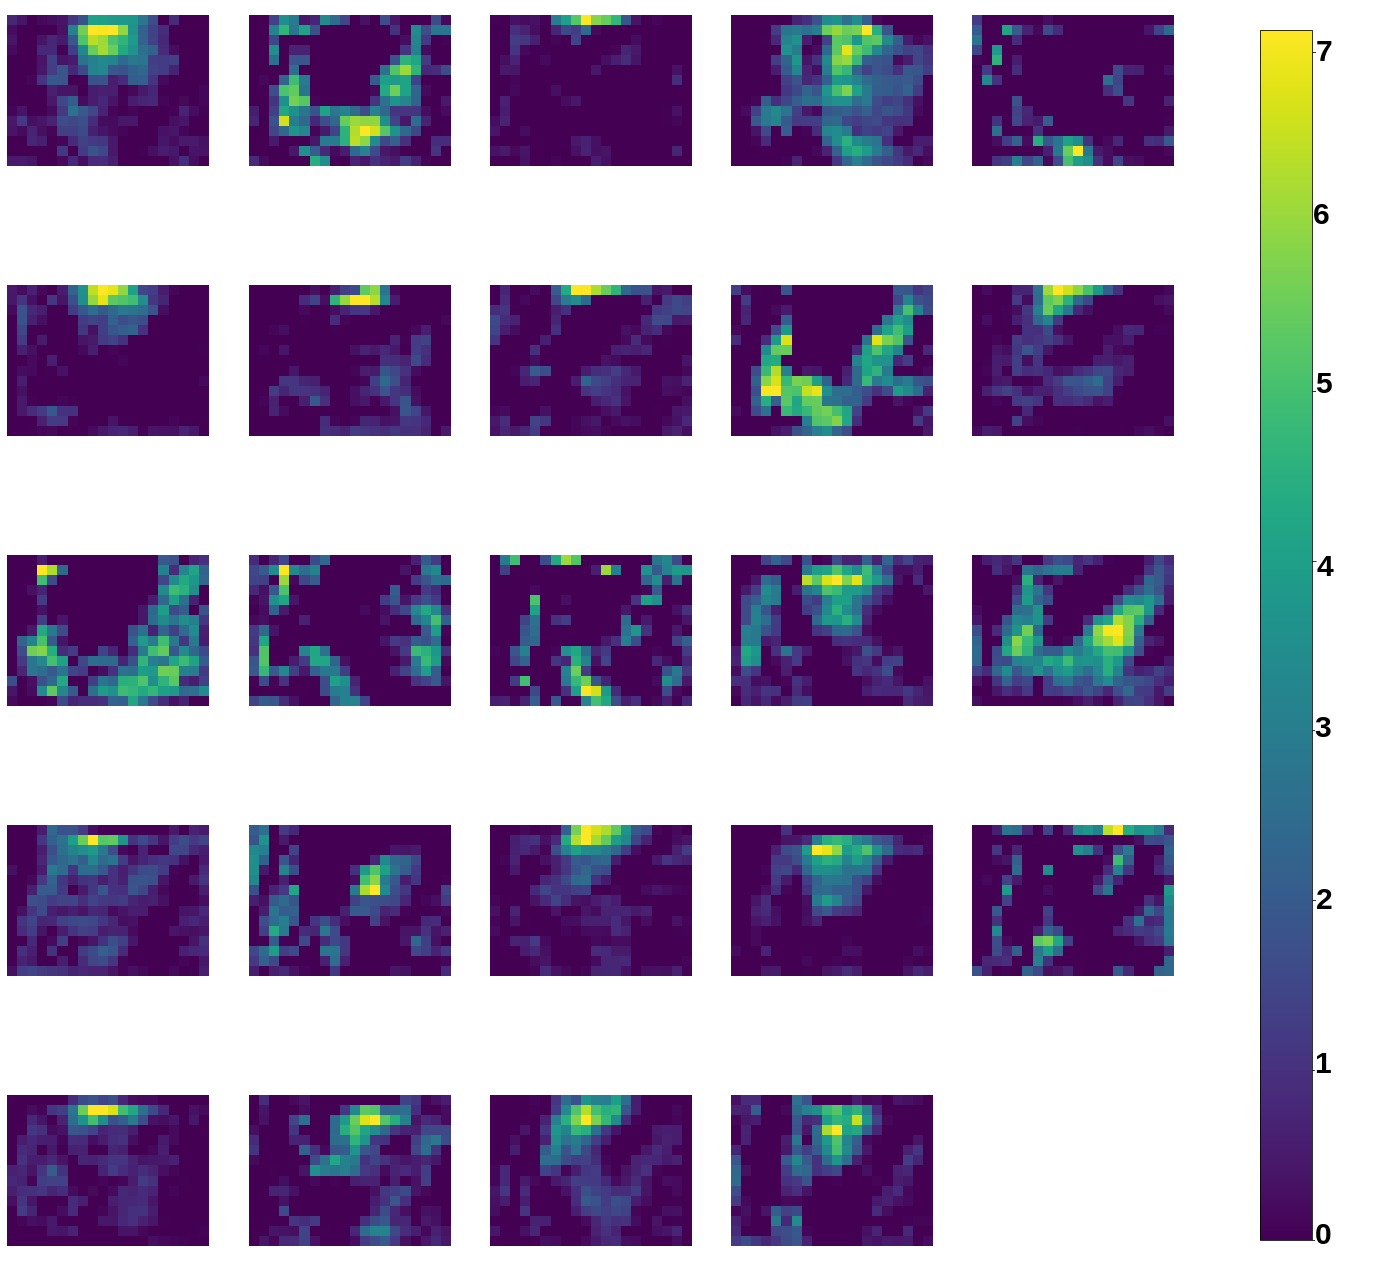
\includegraphics[scale=0.35]{e_conv_154}	
	\caption{Jedenasta warstwa konwolucyjna z 24 filtrami.}\label{fig:e_conv_154}
\end{figure}

\begin{figure}[h!]
	\centering
	\centering
		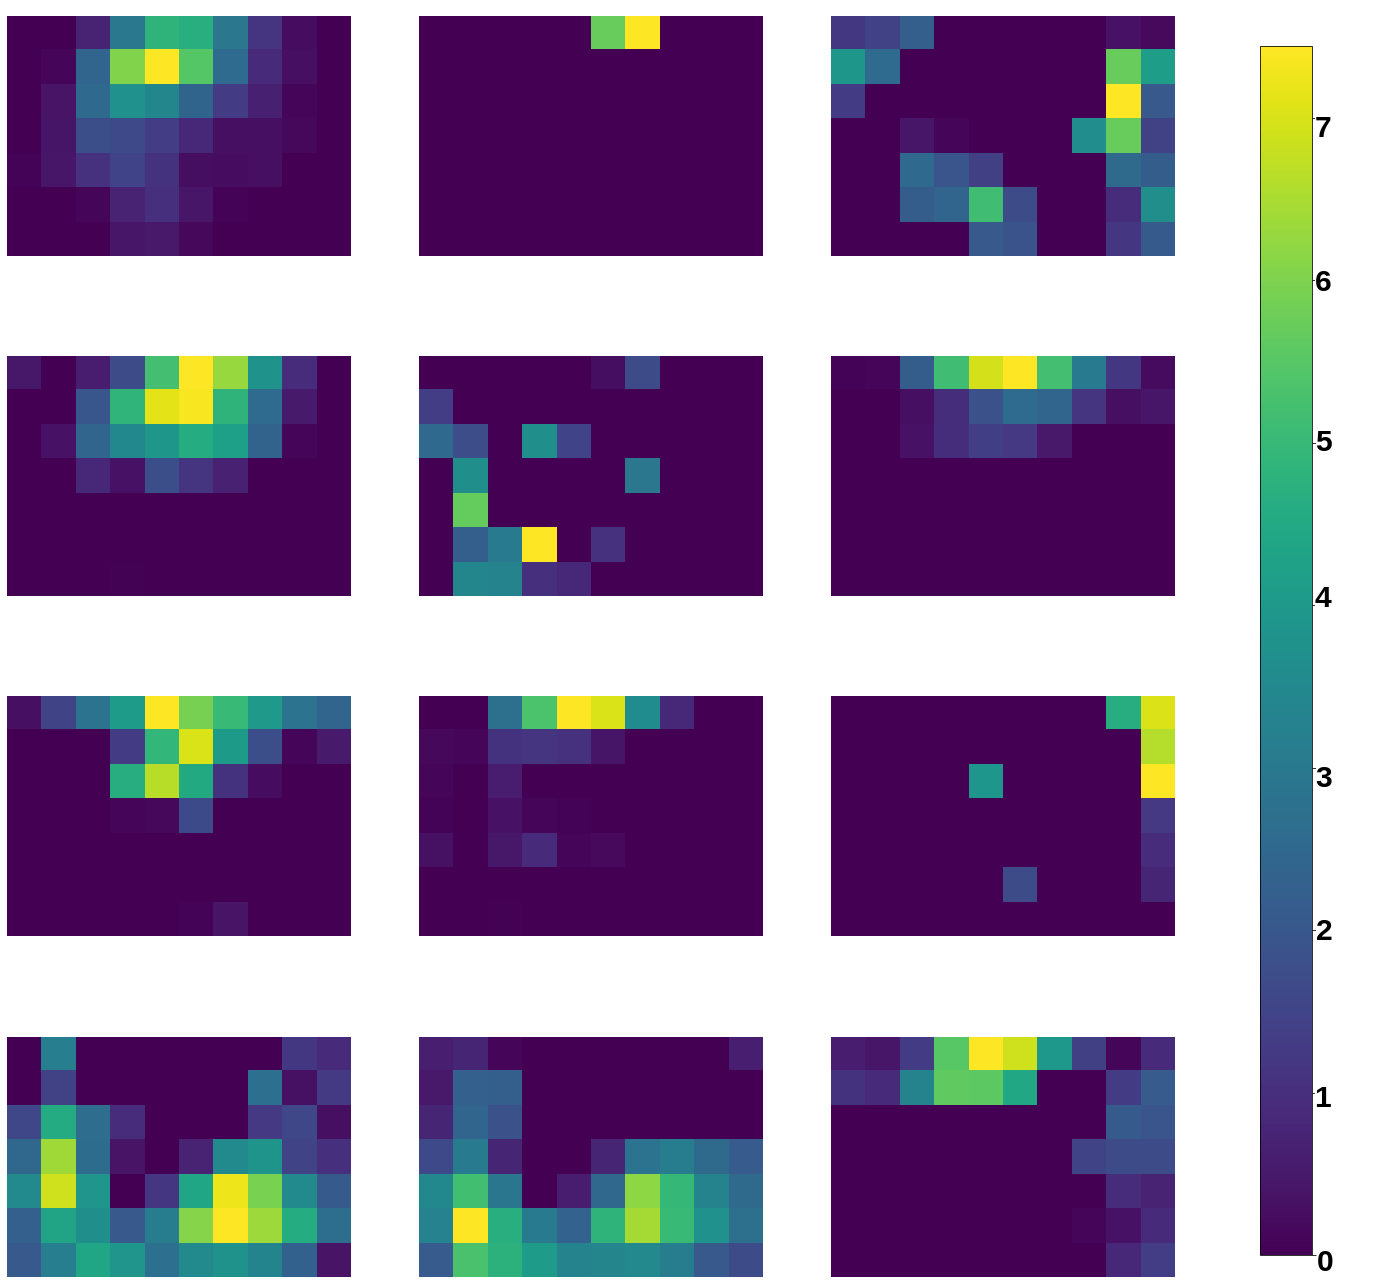
\includegraphics[scale=0.35]{e_conv_156}	
	\caption{Trzynasta i ostatnia warstwa konwolucyjna z 12 filtrami.}\label{fig:e_conv_156}
\end{figure}

\clearpage  
W celu zbadania jakie dokładnie piksele i w jakim stopniu decydują o zaklasyfikowaniu ramki do danej klasy można stworzyć mapę aktywacji na podstawie wag modelu. W ten sposób można stwierdzić czy klasyfikacja przebiega na podstawie oczekiwanych cech. Jest to ważna część weryfikacji, gdyż sieć neuronowa może działać z wysoką skutecznością z powodu cechy bazy danych nie branej pod uwagę przy doborze zdjęć, na przykład charakterystyczne tło \cite{Mller2012IntroductionPA}. Należy wybrać losowo ramkę z bazy, sprawdzić do jakiej klasy sieć ją przypisuje i dla tej klasy pobrać wektor wag z ostatniej warstwy konwolucyjnej sieci. Następnie 
% superimposed_heatmap_e
% heatmap_e